\documentclass[12pt]{article}
\usepackage{hyperref}
\usepackage[utf8]{inputenc}
\usepackage[T1]{fontenc}
\usepackage{graphicx}
\begin{document}
\section*{Rømmegrøt, 30.12.2018}
\begin{itemize}
\item Oppskrift:
  \begin{itemize}
  \item F{\o}lgte følgende
    \href{https://www.matprat.no/oppskrifter/tradisjon/rommegrot/}{oppskrift}
    med 3~dl seterr{\o}mme.  
  \end{itemize}
\item Kommentarer:
  \begin{itemize}
  \item Holdt på å glemme å glemme saltet.        
  \item Tok ganske lang tid for at smør skulle piple ut og
    når det f{\o}rst gjorde det, var det når nærmest umulig
    å fjerne det. Mulig at 1) det var for lite grøt eller
    2) at jeg ventet for kort tid. Uansett, Grøten bar på
    ingen måte preg av å ha for mye fett.
  \end{itemize}
\item Konklusjon:
  \begin{itemize}
  \item Smakte ganske godt, i grunnen få ting jeg ville endret.
  \end{itemize}
\end{itemize}
\centering
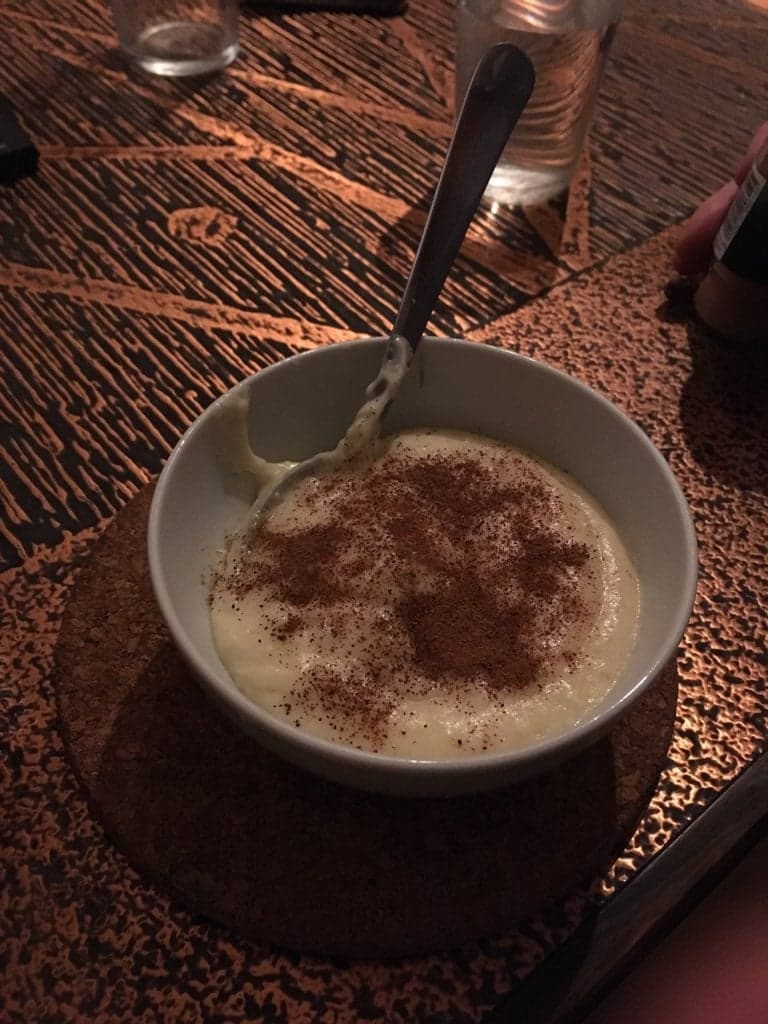
\includegraphics[width=0.33\textwidth]{30-12-2018.jpg}
\end{document}

